%\documentclass[aps,a4paper,12pt]{revtex4}
\documentclass[a4paper,12pt]{article}
\usepackage[top=1cm,,bottom=2cm,left=1.5cm,right=1.5cm]{geometry}
%\RequirePackage[T1]{fontenc}
%\RequirePackage{times}
\usepackage{fancyhdr}
\usepackage{setspace}
\usepackage{amsfonts}
\usepackage{amsmath}
\usepackage{amssymb}
\usepackage{graphicx,epstopdf}
%\usepackage{hyperref}
%\usepackage{color}
\usepackage{xcolor}
\usepackage{graphicx}
\usepackage{animate,subfigure}
\usepackage{caption}

%\pagestyle{fancy}
%\renewcommand{\headrulewidth}{0pt}
%\cfoot{\thepage}


%\renewcommand{\figurename}{Figure}


\begin{document}
% Use default fonts from CJK (see below)

%\maketitle



\begin{spacing}{1.0}

\begin{flushleft}

\includegraphics[scale=1.0]{fudan-logo}
\rule{\textwidth}{0.4pt}
\end{flushleft}


\noindent Dear Editor:

\bigskip

\noindent We are submitting our manuscript entitled ``Observation of optical vortices in momentum space" by Yiwen Zhang et al. for your consideration as a Letter in Nature, in which we made the first experimental observation of \textbf{vortices in momentum space}.

\bigskip

\noindent A vortex is the most fundamental topological excitation in nature. But vortices have been known exclusively in the real space, including hair whorls, plughole spins of water, angular-momentum beams, and defects in liquid crystals and the Kosterlitz--Thouless vortex in superconductors and superfluids (Nobel 2016).

\noindent Our work is significant in several aspects:
\begin{enumerate}
  \item This is the first experiment demonstrating the robust existence of vortices in the momentum space instead of the common real-space vortices, and revealing the topological nature of bound states in continuum (BICs) with diverging lifetime..
  \item The polarization vortex we observe is a unique feature for photons of vector fields. This new topological phenomenon has rich properties beyond the current topological band theory developed for electrons of scalar fields.
  \item Such momentum-space polarization vortices are actually common in 2D photonic lattices but have never been experimentally observed due to a lack of knowledge and proper instrumentation. For this observation in a plasmonic crystal, we introduced and homemade a powerful polarization-resolved momentum-space imaging spectroscopy. This new methodology will be very useful for a wide range of photonic systems.
\end{enumerate}

\noindent We believe this work will generate strong interests from the broad physics and optics communities, and is especially important for the currently very active fields of topological photonics, bound states in continuum, plasmonics, photonic crystals, and vector and angular-momentum beams.

\bigskip

\noindent Best regards,

\noindent Yiwen Zhang, Ang Chen, Wenzhe Liu, Chia Wei Hsu, Fang Guan, Xiaohan Liu, Lei Shi, Ling Lu, Jian Zi

%\begin{figure}[h]
%\centering
%\animategraphics[width=13cm,autoplay,loop]{8}{animation_}{1}{18}
%\end{figure}

%\renewcommand{\figurename}{}

\begin{figure}[h]
\centering
\subfigure{
\begin{minipage}{6cm}
\centering
\caption*{\small\textsf{\quad\quad Measured band structure}}
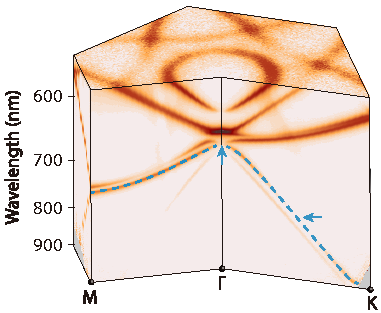
\includegraphics[scale=1]{fig-dispersion}
\end{minipage}
}
\quad\quad
\subfigure{
\begin{minipage}{6cm}
\centering
\caption*{\small\textsf{Vortices observed in momentum space (animation in Acrobat Reader)}}
\animategraphics[scale=1,autoplay,loop]{8}{./animation-figs/animation_c6v_}{1}{18}
\end{minipage}
}
\end{figure}

\newpage

\begin{flushleft}
\textbf{List of potential reviewers}
\end{flushleft}


\footnotesize{
\begin{flushleft}
\begin{tabular}{lll}
  % after \\: \hline or \cline{col1-col2} \cline{col3-col4} ...
  Prof. Naoto Nagaosa  & The University of Tokyo  & nagaosa@appi.t.u-tokyo.ac.jp \\
  Prof. Marco Loncar & Harvard University  & loncar@seas.harvard.edu \\
  Prof. Boubacar Kant\'{e} & University of California San Diego   & bkante@ucsd.edu \\
  Prof. Yuri S. Kivshar & Australian National University & yuri.kivshar@anu.edu.au \\
  Prof. Mikael C. Rechtsman \quad\quad  & The Pennsylvania State University & mcrworld@psu.edu \\
  Prof. Shanhui Fan & Stanford University & shanhui@stanford.edu \\
  Prof. C. T. Chan & Hong Kong University of Science and Technology \quad\quad  & phchan@ust.hk \\
\end{tabular}
\end{flushleft}}

\end{spacing}

\end{document}
